%
% Capa
%

\thispagestyle{empty}

{\sffamily\centering\Large


\includegraphics[scale=0.25]{modelo/UFF_brasao.png}

~\vspace{2cm}

Universidade Federal Fluminense

\vspace{\fill}

{\huge\TITULO}

\vspace{3.5cm}

{\LARGE\AUTOR}

\vspace{\fill}


{\large Niterói }


{\large  July 2023}


}

\clearpage

%
% Folha de rosto
%

\thispagestyle{empty}

{\sffamily\centering\Large

~\vspace{\fill}

{\huge\TITULO}

\vspace{3.5cm}

{\LARGE\AUTOR}

\vspace{3.5cm}

{\normalsize\raggedleft
\begin{minipage}{210pt}
Dissertação submetida ao Programa de Pós-Graduação
em Matemática da Universidade Federal Fluminense
como requisito parcial para a obtenção do grau de
Doutor em Matemática.
\end{minipage}
}

\vspace{3.5cm}

Advisor: \ORIENTADOR

\vspace{\fill}

{\large Niterói }


{\large  July 2023}


}

\clearpage

\thispagestyle{empty}

{\centering 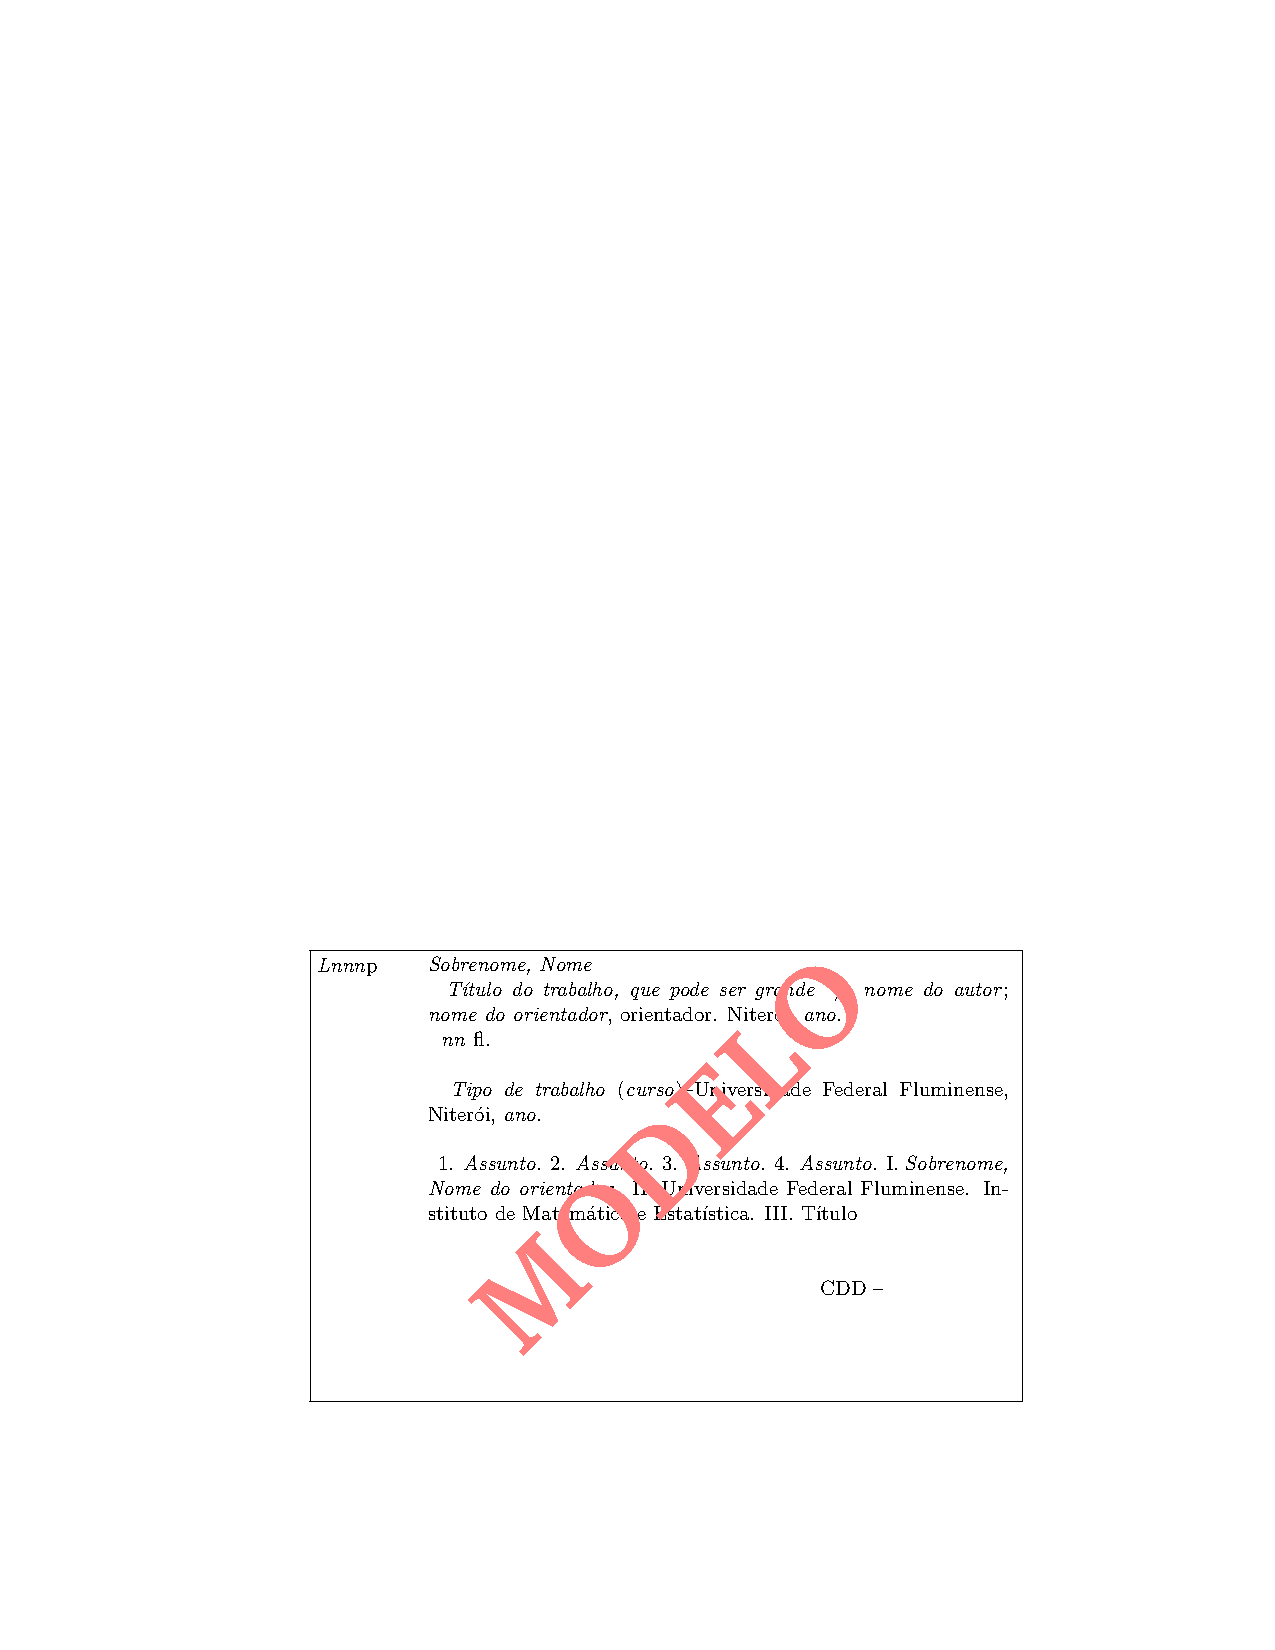
\includepdf{modelo/ficha_catal_modelo}}

\clearpage

\thispagestyle{empty}

{\sffamily\centering

\textbf{Dissertação de Doutorado da Universidade Federal Fluminense}

\vspace{1cm}

 por

\vspace{1cm}

\textbf{\AUTOR}

\vspace{1.5cm}

apresentada ao Programa de Pós-Graduação em Matemática como requesito parcial para a obtenção do grau de

\vspace{1.5cm}

\textbf{Doutor/Mestre em Matemática}

\vspace{1.5cm}

Título da tese:


\hrulefill

\begin{minipage}{0.8\textwidth}
\centering
\textbf{\TITULO}
\end{minipage}
~\vspace{5pt}
\hrule

\vspace{1cm}

\textit{Defendida publicamente em XX julho de 2023.}

\vspace{1cm}

{\raggedright Diante da banca examinadora composta por:}

~\vspace{5pt}

%
% Liste os nomes por ordem alfabética
\begin{tabular}{lll}
  \ORIENTADOR & UFF & Orientador\\
  Simon Chiossi & UFF & Examinador\\
  Thiago Fassarela & UFF & Examinador\\
  Henrique Bursztyn & IMPA & Examinador\\
  Cristián Ortiz & USP & Examinador\\
\end{tabular}

~\vspace{\fill}

}

\clearpage

\thispagestyle{empty}

{
{\centering\textbf{DECLARAÇÃO DE CIÊNCIA E CONCORDÂNCIA DO(A) ORIENTADOR(A)}}

~\vspace{2cm}

Autor(a) da Dissertação: \AUTOR

Data da defesa: XX/07/2023

Orientador(a): \ORIENTADOR

\vspace{2cm}

Para os devidos fins, declaro \textbf{estar ciente} do conteúdo desta \textbf{versão corrigida} elaborada em atenção às sugestões  dos membros da banca examinadora na sessão de defesa do trabalho, manifestando-me \textbf{favoravelmente} ao seu encaminhamento e publicação no \textbf{Repositório Institucional da UFF}.

~\vspace{1cm}

{\raggedright Niterói, XX/03/2023.}

~\vspace{1cm}

\begin{center}
\begin{minipage}{200pt}
\centering
	\hrule

	Nome do orientador(a)
\end{minipage}
\end{center}


}

\clearpage

\thispagestyle{empty}

{

~\vspace{\fill}

\raggedleft
Opcional para esta e aquela pessoa\\
e ainda outra pessoa\\
}

\clearpage

\thispagestyle{empty}

{

\sffamily

{\Large \centering

  AGRADECIMENTOS

}

~\vspace{1cm}

Agradeço a mim mesmo (ou a mais gente). Esta parte é opcional


Agradecimento às agências de fomento --- esta parte \textbf{NÃO É OPCIONAL!}


\textbf{Todas} as teses devem ter o seguinte agradecimento:

\begin{center}
\fbox{
\begin{minipage}{300pt}
O presente trabalho foi realizado com apoio da Coordenação de Aperfeiçoamento de Pessoal de Nível Superior - Brasil (CAPES) - Código de Financiamento 001.
\end{minipage}
}
\end{center}

No caso de bolsa CAPES, sugere-se acrescentar um agradecimento à CAPES pela bolsa. No caso de bolsas de outras agências deve ser verificada quais as regras da agência em particular. Em geral, sugere-se o seguinte: Esse trabalho foi apoiado com uma bolsa de mestrado/doutorado da/do nome da agência, número do processo da bolsa. Outra possibilidade e agradecer a agência em questão a bolsa, mencionando o número do processo ao final.

}

\clearpage

\thispagestyle{empty}

{

	\sffamily

	{\Large	\centering

		RESUMO

	}

~\vspace{1cm}

\lipsum[1-2]

}

\clearpage

\thispagestyle{empty}

{

	\sffamily

	{\Large\centering

		ABSTRACT

	}

~\vspace{1cm}

\kant[1-2]

}
